\chapter{Конструкторский раздел}%
\label{cha:konstruktorskii_razdel}

% В данном разделе рассматривается структура программного обеспечения.

\section{Последовательность преобразований}

На рисунках \ref{img:idef01} и \ref{img:idef02} представлена последовательность преобразований.

\begin{figure}[H]
    \centering
    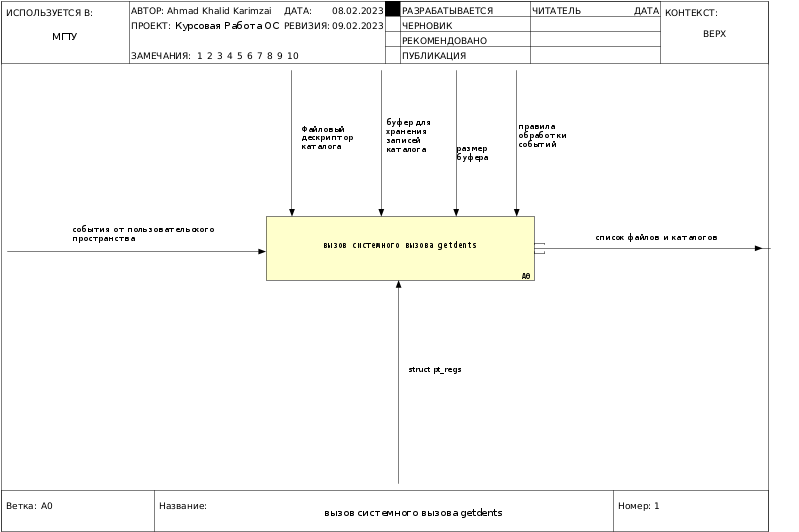
\includegraphics[scale=0.65]{idef/01_A0.png}
    \caption{Нулевой уровень преобразований}\label{img:idef01}
\end{figure}

\begin{figure}[H]
    \centering
    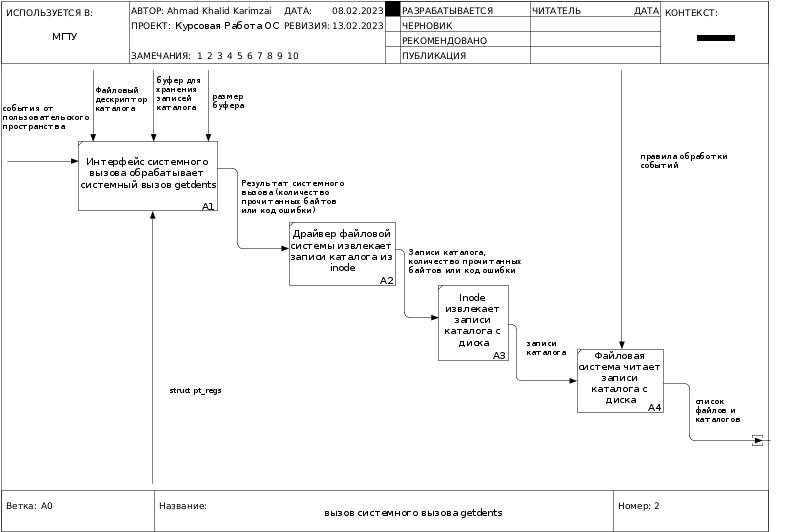
\includegraphics[scale=0.65]{idef/02_A0.png}
    \caption{Первый уровень преобразований}\label{img:idef02}
\end{figure}

\section{Состав загружаемый модуль ядра}%
\label{sec:sostav_programmnogo_obespecheniia}

В состав разработанного программного обеспечения входит один загружаемый модуль ядра, который перехватывает системный вызов getdents64 и функции tcp4\_seq\_show, udp4\_seq\_show, tcp6\_seq\_show, udp6\_seq\_show.

\section{Структура \texttt{struct ftrace\_hook}}

В листинге \ref{lst:ftrace_hook} представлено объявление структуры \texttt{struct ftrace\_hook}, которая описывает каждую перехватываемую функцию.\\

\begin{lstlisting}[label=lst:ftrace_hook, caption=Листинг структуры ftrace\_hook, language=c]
struct ftrace_hook {
	const char *name;
	void *function;
	void *original;
	
	unsigned long address;
	struct ftrace_ops ops;
};
\end{lstlisting}


Необходимо заполнить только первые три поля:

\begin{itemize}
	\item name – имя перехватываемой функции;
	\item function – адрес функции обёртки, вызываемой вместо перехваченной функции;
	\item original – указатель на перехватываемую функцию.
\end{itemize}

Остальные поля считаются деталью реализации. Описание всех перехватываемых были собраны в массив.

\begin{lstlisting}[label=lst:ftrace-array, caption=Объявление массива перехватываемых функций и специальный макрос для его инициализации, language=c]
static struct ftrace_hook	hooks[] = {
	{
		.name = ("udp4_seq_show"),
		.function = (hook_udp4_seq_show),
		.original = &(orig_udp4_seq_show)
	},
	{
		.name = ("udp6_seq_show"),
		.function = (hook_udp6_seq_show),
		.original = &(orig_udp6_seq_show)
	},
	{
		.name = ("tcp4_seq_show"),
		.function = (hook_tcp4_seq_show),
		.original = &(orig_tcp4_seq_show),
	},
	{
		.name = ("tcp6_seq_show"),
		.function = (hook_tcp6_seq_show),
		.original = &(orig_tcp6_seq_show),
	},
	{
		.name = ("__x64_sys_getdents64"),
		.function = (hacked_getdents64),
		.original = &(orig_getdents64),
	},
	{
		.name = ("__x64_sys_getdents"),
		.function = (hacked_getdents),
		.original = &(orig_getdents),
	},
};
\end{lstlisting}


\section{Алгоритм перехвата системного вызова}

На риснуке \ref{fig:ftrace_algo} представлена схема алгоритма перехвата системных вызовов на примере \texttt{sys\_clone}.

\begin{figure}[h]
	\begin{center}
		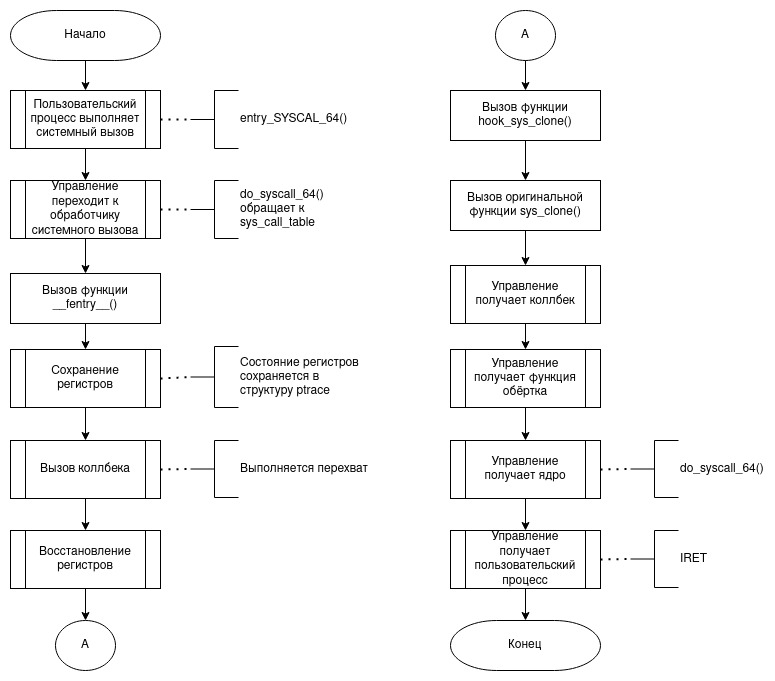
\includegraphics[scale=0.6]{img/ftrace_algo.jpg}
	\end{center}
	\caption{Алгоритм перехвата системного вызова}
	\label{fig:ftrace_algo}
\end{figure}

\begin{enumerate}
	\item Пользовательский процесс выполняет инструкцию \texttt{SYSCALL}. С помощью этой инструкции выполняется переход в режим ядра и управление передаётся низкоуровневому обработчику системных вызовов \texttt{entry\_SYSCALL\_64()}. Этот обработчик отвечает за все системные вызовы 64-битных программ на 64-битных машинах.
	
	\item Управление переходит к обработчику системного вызова. Ядро передаёт управление функции \texttt{do\_syscall\_64()}. Эта функция обращается к таблице обработчиков системных вызовов \texttt{sys\_call\_table} и с помощью неё вызывает конкретный обработчик системного вызова -- \texttt{sys\_clone()}.
	
	\item Вызывается \texttt{ftrace}. В начале каждой функции ядра находится вызов функции \texttt{\_\_fentry\_\_()}, реализованная фреймворком \texttt{ftrace}. Перед этим состояние регистров сохраняется в специальную структуру \texttt{pt\_regs}.
	
	\item \texttt{ftrace} вызывает разработанный коллбек.
	
	\item Коллбек выполняет перехват. Коллбек анализирует значение  \texttt{parent\_ip} и выполняет перехват, обновляя значение регистра \texttt{rip} (указатель на следующую исполняемую инструкцию) в структуре \texttt{pt\_regs}.
	
	\item \texttt{ftrace} восстанавливает значение регистров с помощью структуры \texttt{pt\_regs}. Так как обработчик изменяет значение регистр \texttt{rip} -- это приведёт к передачу управления по новому адресу.
	
	\item Управление получает функция обёртка. Благодаря безусловному переходу, управление получает наша функция \texttt{hook\_sys\_clone()}, а не оригинальная функция \texttt{sys\_clone()}. При этом всё остальное состояние процессора и памяти остаётся без изменений -- функция получает все аргументы оригинального обработчика и при завершении вернёт управление в функцию \texttt{do\_syscall\_64()}.
	
	\item Функция обёртка вызывает оригинальную функцию. \\Функция \texttt{hook\_sys\_clone()} может проанализировать аргументы и контекст системного вызова и запретить или разрешить процессу его выполнение. В случае его запрета, функция просто возвращает код ошибки. Иначе -- вызывает оригинальный обработчик \texttt{sys\_clone()} повторно, с помощью указателя \texttt{real\_sys\_clone}, который был сохранён при настройке перехвата.
	
	\item Управление получает коллбек. Как и при первом вызове \texttt{sys\_clone()}, управление проходит через \texttt{ftrace} и передается в коллбек.
	
	\item Коллбек ничего не делает. В этот раз функция \texttt{sys\_clone()} вызывается разработанной функцией \texttt{hook\_sys\_clone()}, а не ядром из функции \texttt{do\_syscall\_64()}. Коллбек не модифицирует регистры и выполнение функции \texttt{sys\_clone()} продолжается как обычно.
	
	\item Управление передаётся функции обёртке.
	
	\item Управление передаётся ядру. Функция \texttt{hook\_sys\_clone()} завершается и управление переходит к \texttt{do\_syscall\_64()}.
	
	\item Управление возвращает в пользовательский процесс. Ядро выполняет инструкцию \texttt{IRET}, устанавливая регистры для нового пользовательского процесса и переводя центральный процессор в режим исполнения пользовательского кода.
\end{enumerate}

\section{Скрытие файлы и каталоги}%
\label{sec:skrytie_protsessov}

В результате анализа системных вызовов, которые использует утилита ls, с помощью утилиты strace, описание которой представлено в аналитическом разделе, было выявлено, что каждая операция по файлы и каталоги требует использование системного вызова getdents64 (или её альтернативной реализации для более старых файловых систем~--- getdents). Именно этот системный вызов было решено заменить собственным обработчиком.

В листинге~\ref{lst:getdents} представлен прототип системного вызова getdents.
\begin{lstlisting}[language=c,caption={Прототип системного вызова getdents},label=lst:getdents]
int getdents(unsigned int fd, struct linux_dirent *dirp, unsigned int count);
int getdents64(unsigned int fd, struct linux_dirent64 *dirp, unsigned int count);
\end{lstlisting}

Системный вызов getdents читает несколько структур linux\_dirent из каталога, на который указывает fd в область памяти, на которую указывает dirp. Параметр count является размером этой области памяти.

Для использования системного вызова getdents необходимо самостоятельно определить структуру linux\_derent (для getdents64 аналогичная структура уже определена в доступном для пользователя заголвочном файле), которая представлена на листинге~\ref{lst:linux_dirent}.
\begin{lstlisting}[language=c,caption={Структура linux\_dirent},label=lst:linux_dirent]
struct linux_dirent {
    unsigned long	d_ino;
    unsigned long	d_off;
    unsigned short	d_reclen;
    char		    d_name[1];
};
\end{lstlisting}

В модифицированной версии функции getdents64 происходит вызов оригинального системного вызова, после которого происходит проверка на то, соответствует название текущим или предыдущим каталогом. Если не это так, то происходит скрытия этого файла, что приводит и к скрытию всех файлы и каталоги (от команды ls в частности).

\begin{figure}[H]
    \centering
    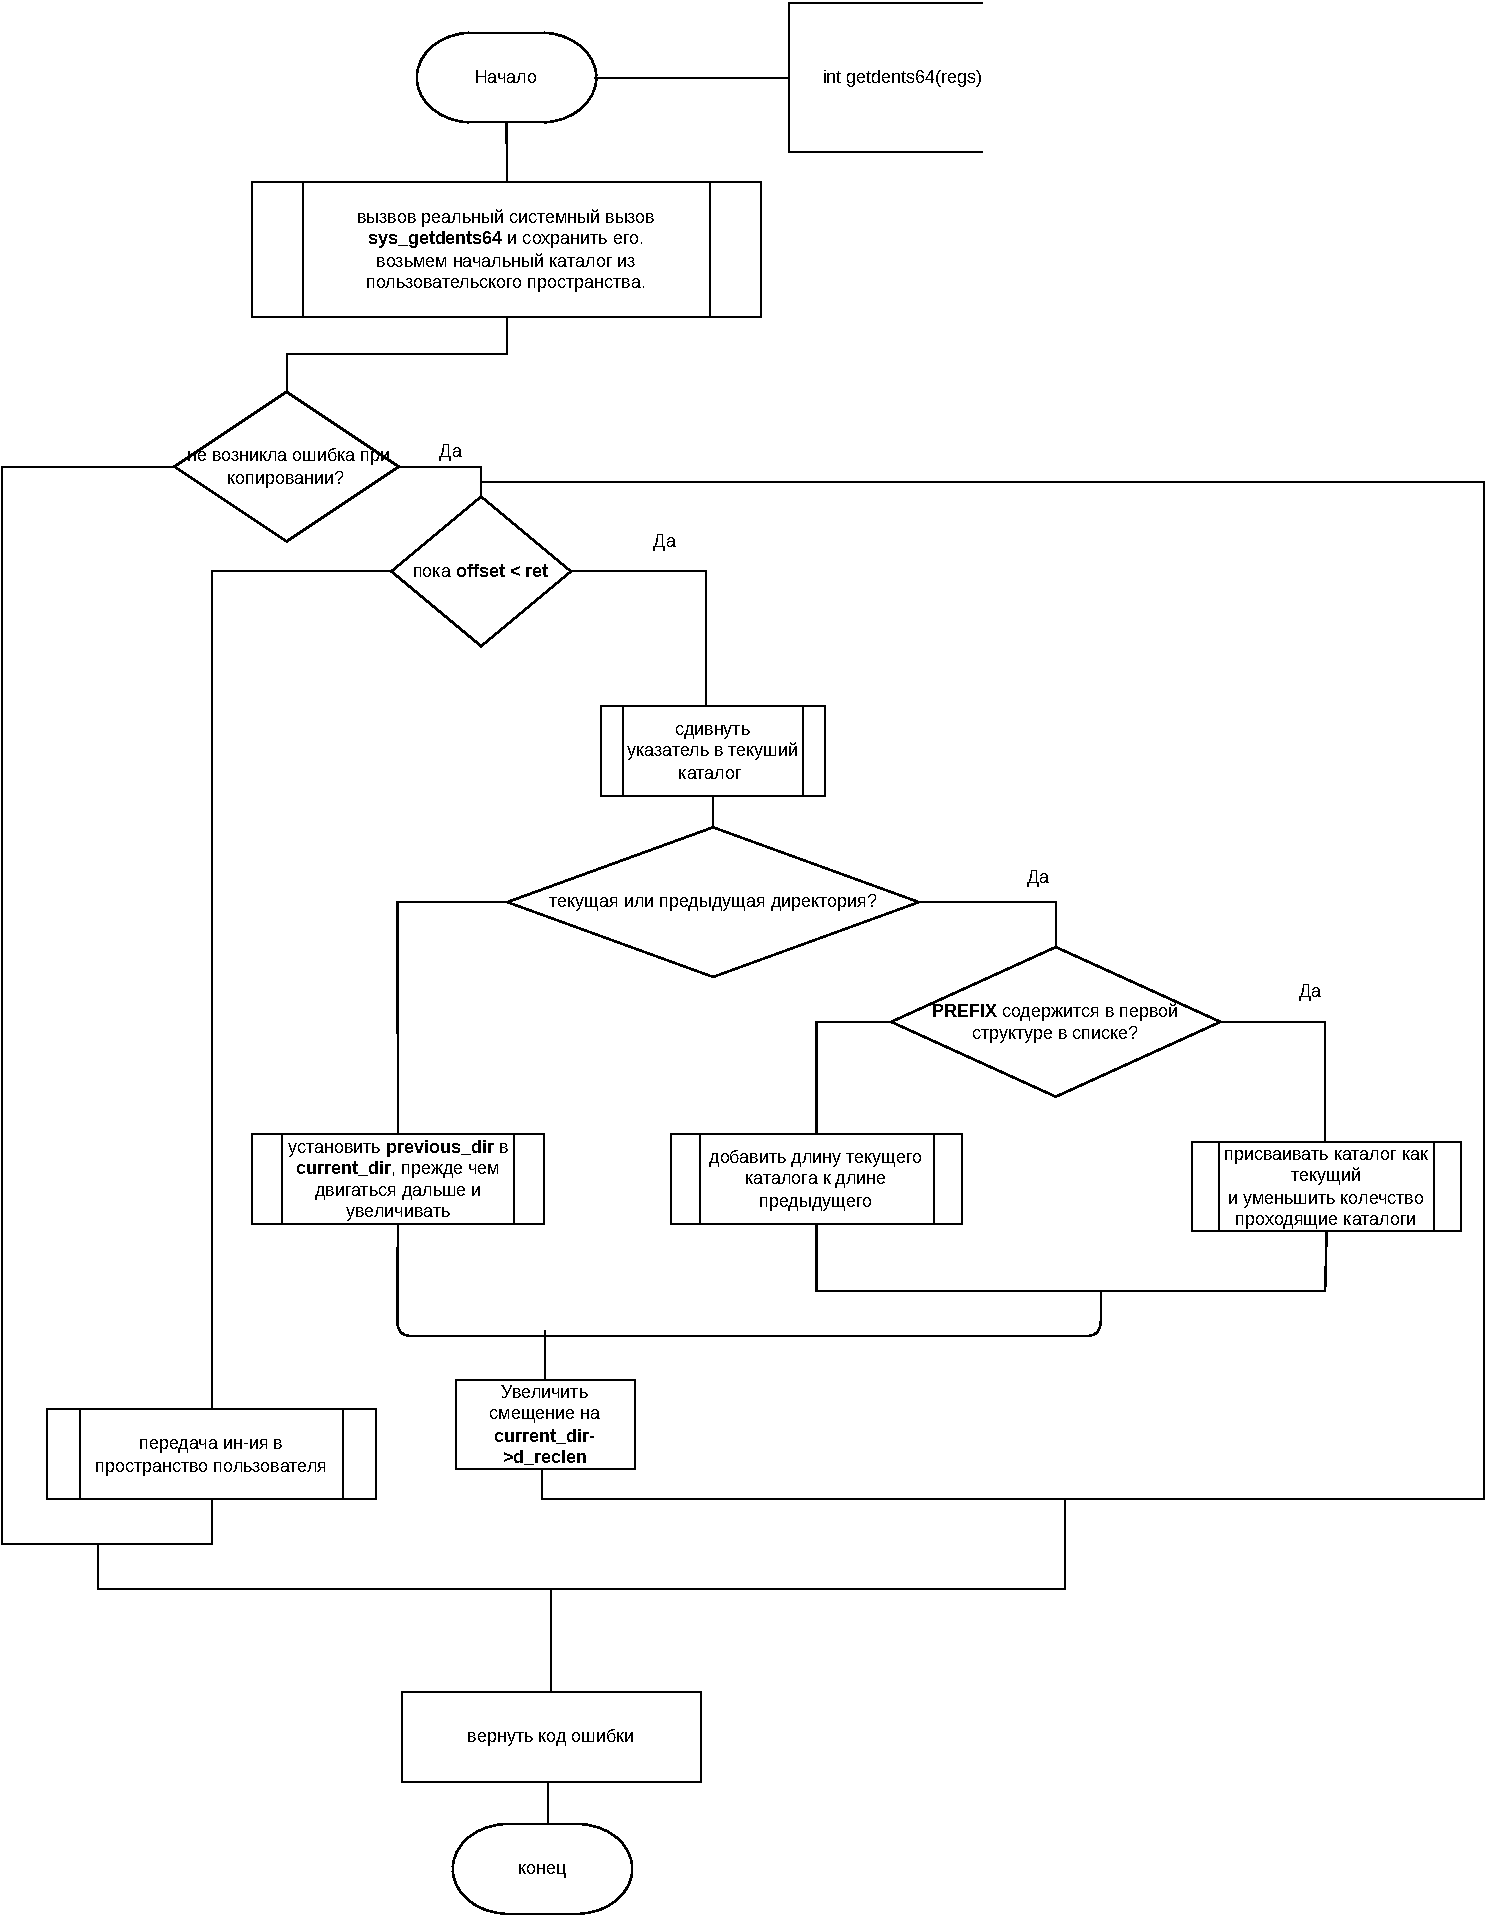
\includegraphics[scale=0.65]{pdf/os_dirent.pdf}
    \caption{Схема алгоритма скрытия файлы и каталоги}\label{img:proc_hide_scheme}
\end{figure}

\section{Скрытие сетевых сокетов}%
\label{sec:skrytie_setevykh_soketov}

Как показал анализ утилиты netstat при помощи программы strace, для отображения сетевых сокетов выполняется чтение /proc/net/tcp (tcp6, udp, udp6).

Для работы с файлами виртуальной файловой системы существуют специальный интерфейс~--- файловые последовательности, описываемые структурой struct seq\_file.

Для работы с файловыми последовательностями необходимо реализовать специальные функции. Для упомянутых выше файлов в ядре есть соответствующии им имплементации: tcp4\_seq\_show, udp4\_seq\_show, tcp6\_seq\_show, udp6\_seq\_show. В листинге~\ref{lst:tcp4_seq_show} представлен прототип одной из них.
\begin{lstlisting}[language=c,caption={Прототип tcp4\_seq\_show},label=lst:tcp4_seq_show]
int tcp4_seq_show(struct seq_file *seq, void *v);
\end{lstlisting}

Среди полей структуры struct seq\_file есть буфер buf, в который происходит запись содержимого файла. За каждый вызов упомянутой функции в этот буфер помещается новая строка.

В рассматриваемом случае, эта строка содержит информацию о сетевом подключении. Чтобы скрыть сетевой сокет, данную строку необходимо удалить из буфера.

\begin{figure}[H]
    \centering
    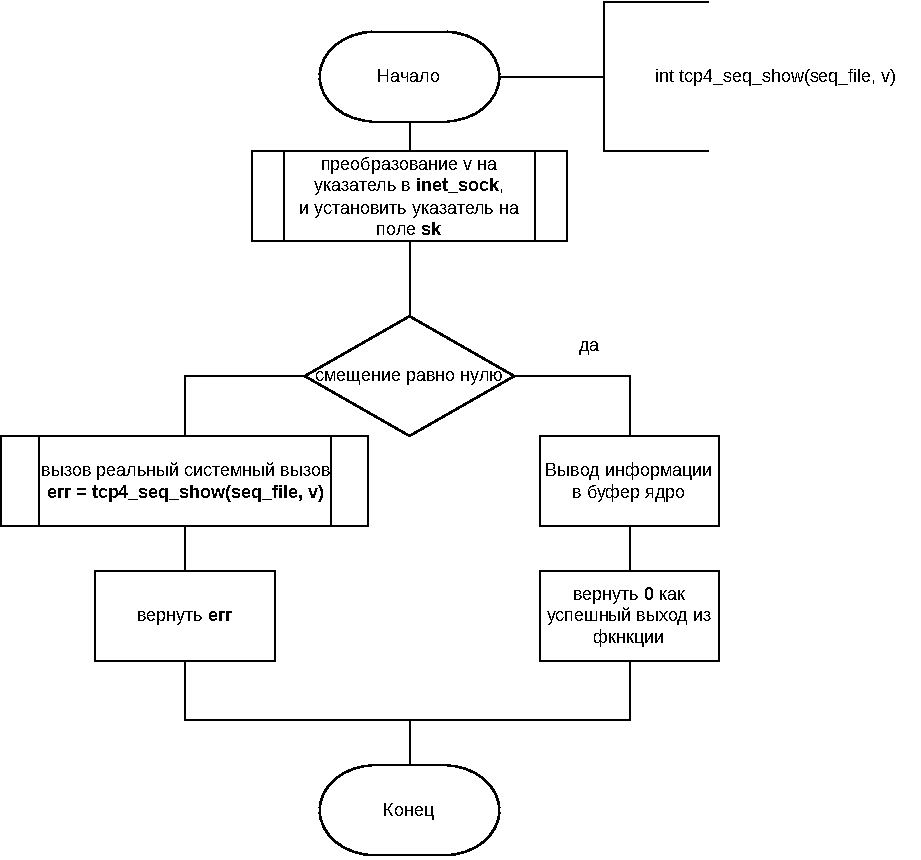
\includegraphics[scale=0.65]{pdf/os_net.pdf}
    \caption{Схема алгоритма скрытия открытых сетевых сокетов}\label{img:net_hide_scheme}
\end{figure}

%\section*{Выводы}%
%\label{sec:vyvody}

%В данном разделе был рассмотрен процесс проектирования структуры программного обеспечения.
